\documentclass[USenglish,limits]{report}
\usepackage{mathsim}
\svnid{$Id$}
\usepackage[notref,notcite,final]{showkeys}
%\usepackage{hyperref}
\usepackage[math]{iwona}
\usepackage[backend=bibtexu,style=alphabetic]{biblatex}
\addbibresource{all}

\title{\textbf{Notes on Applied Mathematics}
\\[5mm]
{\large Interative Methods and Preconditioning}}
\author{Guido Kanschat}
\date{\today\\[5mm]Revision: \svnrev}

%\renewcommand{\thechapter}{B.\arabic{chapter}}

\makeindex
\begin{document}
\maketitle

\section*{Preface}
These notes are a short presentation of the material presented in my
lecture. They follow the notes by Rannacher (Numerik 1 in German)
as well as the books by Hairer, Nørsett, and
Wanner~\cite{HairerNorsettWanner93} and Hairer and
Wanner~\cite{HairerWanner10}. Furthermore, I used the book by
Deuflhard and Hohmann~\cite{DeuflhardBornemann08}. Historical remarks
are in part taken from the article by Butcher~\cite{Butcher96}.

I am always thankful for hints and errata. But please verify that you
have the latest version, which is available on github.

My thanks go to David Stronczek, Markus Schubert, and Dörte Jando for their help
writing and translating these notes.

\clearpage
\section*{Index for shortcuts}
\begin{tabular}{ll}
  IVP & Initial value problem, s. definition~\ref{Definition:awa} on page~\pageref{Definition:awa}\\
  BDF & Backward differencing formula, s. example~\ref{ex:lmm:3} on page~\pageref{ex:lmm:3}\\
  ODE & Ordinary differential equation\\
  DIRK & Diagonal implicit Runge-Kutta method\\
  ERK & Explicit Runge-Kutta method\\
  IRK & Implicit Runge-Kutta method\\
  LMM & Linear multistep method, s. Definition~\ref{Definition:lmm} on
  page~\pageref{ex:lmm:1}\\
  VIE & Volterra integral equation, s. Remark~\vref{remark:volterra}
\end{tabular}

\section*{Index for symbols}
\begin{tabular}{lp{10cm}}
  $\C$ & The set of complex numbers\\
  $e_i$ & The unit vector of $\C^d$ in direction $d$\\
  $\Re$ & Real part of a complex number\\
  $\R$ & The set of real numbers\\
  $\R^d$ & The $d$-dimensional vectorspace of the real $d$-tuple\\
  $u$ & The exact solution of an ODE or IVP\\
  $u_k$ & The exact solution at time step $t_k$\\
  $y_k$ & The discrete solution at time step $t_k$\\
  $\scal(x,y)$ & The Euclidean scalar product in the space $\R^d$ or
  $\C^d$\\
  $\abs{x}$ & The absolute value of a real number, the modulus of a
  complex number, or the Euclidean norm in $\R^d$ or $\C^d$, depending
  on its argument\\
  $\norm{u}$ & A norm in a vector space (with exception of the special
  cases covered by $\abs{x}$)
\end{tabular}

\cleardoublepage

%%% Local Variables: 
%%% mode: latex
%%% TeX-master: "notes"
%%% End: 


\begin{todo}
  Note: yellow boxes indicate text which is missing in the current
  version and will be added soon.
\end{todo}

\tableofcontents

\chapter{Iterative methods in finite and infinite dimensional spaces}

\begin{remark}
  This part of the notes deals with preconditioning of symmetric
  operators, or those, which have a dominating symmetric part. The
  theory of preconditioning methods for nonsymmetric and in particular
  non-normal operators is currently barely developed and thus cannot
  be covered by these notes. 
\end{remark}

\svnid{$Id$}

\section{The Richardson iteration}

\begin{intro}
  As a first example and prototype for all other iterative methods we
  consider Richardson's method, which for matrices and vectors in
  $\R^n$ reads
  \begin{gather}
    \label{eq:richardson:1}
    \vec x^{(k+1)}
    = \vec x^{(k)}
    - \omega_k \bigl(\mat A \vec x^{(k)} - \vec b \bigr).
  \end{gather}
  $\omega_k$ is a relaxation parameter, which can be chosen a priori
  or can be changed in every step. We will for simplicity assume
  $\omega_k = \omega$.
  
  It can be shown easily, that if $\mat A$ is symmetric, positive definite,
  the method converges if $\omega$ is sufficiently small. More
  precisely, let
  \begin{gather}
    \label{eq:richardson:3}
    \lambda
    = \min_{x\in \R^n} \frac{\vec x^T\mat A\vec x}{\vec x^T\vec x},
    \qquad\text{and}\qquad
    \Lambda = \max_{x\in \R^n} \frac{\vec x^T\mat A\vec x}{\vec x^T\vec x}.
  \end{gather}
  Then, the method converges for $0 < \omega < 2/\Lambda$. The optimal
  choice is
  \begin{gather}
    \label{eq:richardson:2}
    \omega = \frac{2}{\lambda+\Lambda},
  \end{gather}
  which leads to a contraction rate of
  \begin{gather}
    \label{eq:richardson:4}
    \rho = \frac{\Lambda-\lambda}{\Lambda+\lambda} =
    \frac{\kappa-1}{\kappa+1} = 1 -\frac2\kappa + \mathcal
    O(\kappa^{-2}),
  \end{gather}
  where $\kappa = \Lambda/\lambda$ is the spectral condition number. 
\end{intro}

\begin{intro}
  The analysis of finite element methods shows that it is beneficial
  to give up the focus on finite dimensional spaces and rather use
  theory that applies to separable Hilbert spaces. If results can
  obtained in this context, they can easily be restricted to finite
  dimensional subspaces and thus become uniform with respect to the
  mesh parameter. Thus, we will first reformulate Richardson's method
  for this case and then derive convergence estimates.
\end{intro}

\begin{intro}
  Elements of an abstract Hilbert space $V$ will be denoted by
  $u,v,w$, etc. On the other hand, coefficient vectors in $\R^n$ are
  denoted by letters $\vec x,\vec y,\vec z$, etc.
\end{intro}

\begin{definition}
  Let $V$ be a Hilbert space with inner product $\scal(.,.)_V$. Let
  $a(.,.)$ be a second bilinear form on $V$. Then, for any right hand
  side $f\in V^*$ and any start vector $u^{(0)}\in V$,
  \define{Richardson's method} is defined by the iteration
  \begin{gather}
    \label{eq:richardson:5}
    \scal(u^{(k+1)},v)_V = \scal(u^{(k)},v)_V
    - \omega_k \bigl(a(u^{(k)},v) - f(v)\bigr), \qquad \forall v\in V.
  \end{gather}
  $\omega_k$ is a suitable \putindex{relaxation parameter}, chosen
  such that the method converges.
\end{definition}

\begin{note}
  The scalar products in~\eqref{eq:richardson:5} become necessary,
  since different from the case in $\R^n$, the result of applying the
  bilinear form $a(.,.)$ to $u^{(k)}$ in the first argument yields a
  linear form on $V$. In order to convert this to a vector in $V$, we
  have to apply the isomorphism induced by the \putindex{Riesz
    representation theorem}.
\end{note}

\begin{theorem}
  \label{theorem:richardson:1}
  Let the bilinear form $a(.,.)$ be bounded and elliptic on $V\times
  V$, namely, let there exist positive constants $\Lambda$ and $\lambda$ such
  that for all $u,v\in V$ there holds
  \begin{gather}
    \label{eq:richardson:6}
    a(u,v) \le \Lambda \norm{u}_V \norm{v}_V,
    \qquad
    a(u,u) \ge \lambda \norm{u}_V^2.
  \end{gather}
  Then, the Richardson iteration~\eqref{eq:richardson:5} converges for
  $\omega_k = \omega \in (0, 2 \lambda/\Lambda^2)$. The optimal
  choice is $\omega$ according to~\eqref{eq:richardson:2}, in which
  case the convergence rate is given by~\eqref{eq:richardson:4}.
\end{theorem}

\begin{proof}
  We define the iteration operator $T$ as the solution operator of
  equation~\eqref{eq:richardson:5}, namely $T u{(k)} := u{(k+1)}$. We
  have to prove that $T$ is a contraction on $V$ under the assumptions
  of the theorem.

  For two arbitrary vectors $u^1, u^2 \in V$, let $w = u^1-u^2$ be
  their difference. Due to linearity, we have $T w = T u^1-T u^2$ and
  \begin{gather*}
    \scal(T w,v)_V = \scal(w,v)_V - \omega a(w,v) = \scal(w-\omega A w,v)_V.
  \end{gather*}
  Using $v=Tw$ as a test function, we obtain
  \begin{align*}
    \norm{Tw}_V^2
    & = \scal(w-\omega A w,w-\omega A w)_V \\
    &= \norm{w}_V^2 - 2\omega a(w,w) + \omega^2 \norm{Aw}_V^2\\
    & \le \norm{w}_V^2 - 2\lambda\omega \norm{w}_V^2
    +  \Lambda^2 \omega^2\norm{w}_V^2\\
    & = \underbrace{\bigl(1-2\lambda\omega
      + \Lambda^2\omega^2\bigr)}_{=:\rho(\omega)} \norm{w}_V^2.
  \end{align*}
  \begin{todo}
    Check the actual convergence!
  \end{todo}
  The function $\rho(\omega)$ is a parabola open to the top, which
  equals one at zero and $2/\Lambda$.
\end{proof}

\begin{note}
  It is clear that the boundedness and ellipticity
  estimates~\eqref{eq:richardson:6} hold for any finite dimensional
  subspace $V_n\subset V$, and thus the convergence
  estimate~\eqref{eq:richardson:4} becomes independent of $n$.
\end{note}  

\begin{note}
  We define an operator $B:V\to V^*$ such that $Bu = b(u,.) :=
  \scal(u,.)_V$. By the Riesz representation theorem, there is a
  continuous inverse operator $B^{-1}: V^*\to V$, which is often
  called \define{Riesz isomorphism}.
\end{note}

\begin{definition}
  When we apply Richardson's method as in~\eqref{eq:richardson:5} on a
  computer, each step involves a multiplication with the matrix $\mat A$,
  but an inversion of the matrix $\mat B$, corresponding to the iteration
  \begin{gather*}
    \mat B \vec x^{(k+1)}
    = \mat B \vec x^{(k)}
    - \omega_k \bigl(\mat A \vec x^{(k)} - \vec b \bigr),
  \end{gather*}
  or equivalently,
  \begin{gather}
    \label{eq:richardson:7}
    \vec x^{(k+1)}
    = \vec x^{(k)}
    - \omega_k \mat B^{-1}\bigl(\mat A \vec x^{(k)} - \vec b \bigr).
  \end{gather}
  The iteration in~\eqref{eq:richardson:7} is commonly referred to as
  \define{preconditioned Richardson iteration} and $\mat B^{-1}$ as the
  \define{preconditioner}. Note that by introducing the iteration in
  its weak form~\eqref{eq:richardson:5}, the preconditioner arrives
  naturally and with necessity.
  
  The goal of this chapter is finding preconditioners $\mat B^{-1}$, or
  equivalently inner products $\scal(.,.)_V$, such that the bilinear
  form $a(.,.)$ is bounded and the condition number
  $\kappa = \Lambda/\lambda$ is small.
  
  In order to reduce (or increase) confusion, we will refer to the
  inner product that we search in order to bund the condition number
  as $b(.,.)$ instead of $\scal(.,.)_V$, this way separating the
  Hilbert space $V$ more clearly from the task of
  preconditioning. Thus, the operator $B$ and the matrix $\mat B$ will
  be associated with a bilinear form $b(.,.)$ and the final version of
  the preconditioned Richardson iteration in the space $V$ is
  \begin{gather}
    \label{eq:richardson:10}
    b(u^{(k+1)},v)_V = b(u^{(k)},v)_V
    - \omega_k \bigl(a(u^{(k)},v) - f(v)\bigr), \qquad \forall v\in V,
  \end{gather}
  or in operator form
  \begin{gather}
    \label{eq:richardson:11}
    u^{(k+1)} = u^{(k)} - \omega_k B^{-1} (A u^{(k)} - f).
  \end{gather}
\end{definition}

\begin{corollary}
  Let the symmetric bilinear forms $a(.,.)$ and $b(.,.)$ in the
  Richardson iteration~\eqref{eq:richardson:10} fulfill the
  \define{spectral equivalence} relation
  \begin{gather}
    \label{eq:richardson:12}
    \lambda b(u,u) \le a(u,u) \le \Lambda b(u,u), \quad \forall u\in V.
  \end{gather}
  Then, if $\omega_k \equiv \omega \in (0,2\Lambda)$, the iteration is
  a contraction on $V$. The optimal contraction number is $\rho$
  according to equation~\eqref{eq:richardson:4} for $\omega$ chosen as
  in~\eqref{eq:richardson:2}.
\end{corollary}

\begin{proof}
  This corollary is equivalent to Theorem~\ref{theorem:richardson:1}
  if the inner product $\scal(.,.)_V$ is replaced by the bilinear form
  $b(.,.)$.
\end{proof}

\begin{notation}
  \index{lambdaBA@$\lambda(B,A)$}
  \index{Lambdaba@$\Lambda(B,A)$}
  In order to distinguish different preconditioners, we will also us
  the notation $\lambda(B, A)$ and $\Lambda(B,A)$ to refer to the
  constants in the norm equivalence~\eqref{eq:richardson:12}.
\end{notation}


\begin{example}
  Let us take the example~\eqref{eq:main:1}.
  By the Poincaré-Friedrichs inequality, $a(.,.)$ is an inner product
  on $V$ and thus we can choose $\scal(.,.)_V = a(.,.)$. In
  particular, $\lambda = \Lambda = 1$ and the optimal choice is
  $\omega = 1$. Then, Richardson's iteration becomes
  \begin{gather*}
    a(u^{(k+1)},v) = a(u^{(k)},v)
    - \bigl(a(u^{(k)},v) - f(v)\bigr) =  f(v), \qquad \forall v\in V,
  \end{gather*}
  which converges in a single step, but we have to solve the original
  equation for $u$. Thus, either the inversion of the matrix $A_n$ is
  trivial on each finite dimensional subspace $V_n$, or the method is
  useless. With usual finite element bases, the latter is true.
\end{example}

\begin{example}
  In the other extreme, we would like to use the $\R^n$ or $L^2$
  inner product on $V_n$ or $V$, such that the Riesz isomorphism is
  easily computable. But then, the bilinear form $a(.,.)$ is unbounded
  on $V$. Thus, while for each finite $n$, the condition number
  $\kappa_n = \Lambda_n/\lambda_n$ exists, it converges to infinity if
  $n\to\infty$.
\end{example}

\begin{todo}
  Show that the condition number grows like $1/h^2$ for finite element
  methods.
\end{todo}

%%% Local Variables: 
%%% mode: latex
%%% TeX-master: "main"
%%% End: 

\svnid{$Id$}

\section{The conjugate gradient method}

\begin{intro}
  Relying on Hilbert space structure more than Richardson's iteration
  is the \define{conjugate gradient method} (cg), since it uses
  orthogonal search directions. Nevertheless, it also relies on
  constructing search directions from residuals, such that a
  \putindex{Riesz isomorphism} enters the same way as before and can
  then be used for preconditioning.
  
  The beauty of the conjugate gradient method is, that it is parameter
  and tuning free, and it converges considerably faster than a linear
  iteration method.
\end{intro}

\begin{definition}
  Let $V$ be a Hilbert space and $V^*$ its dual. The conjugate
  gradient method for an iteration vector $x^{(k)} \in V$ involves the
  residuals $r^{(k)} \in V^*$ as well as the update direction $p^{(k)}
  \in V$ and the auxiliary vector $z^{(k)} \in V$. It consists of the
  steps
  \begin{enumerate}
  \item Initialization: for $f$ and $x^{(0)}$ given, compute
    \begin{xalignat*}{2}
      r^{(0)} &= f- a(x^{(0)},.) \\
      \scal(z^{(0)}, v) &= r^{(0)}(v) & \forall v &\in V \\
      p^{(0)} &= z^{(0)}.
    \end{xalignat*}
    \item Iteration step: for $x^{(k)}$, $r^{(k)}$, $z^{(k)}$, and
      $p^{(k)}$ given, compute
      \begin{xalignat*}2
        \alpha_k &= \frac{r^{(k)}(z^{(k)})}{a(p^{(k)},p^{(k)})} \\
        x^{(k+1)} &= x^{(k)} + \alpha_k p^{(k)} \\
        r^{(k+1)} &= r^{(k)} - \alpha_k a(p^{(k)},.) \\
      \scal(z^{(k+1)}, v) &= r^{(k+1)}(v) & \forall v &\in V \\
      \beta_k &= \frac{r^{(k+1)}(z^{(k+1)})}{r^{(k)}(z^{(k)})}\\
      p^{(k+1)} &= z^{(k+1)} + \beta_k p^{(k)}
      \end{xalignat*}
  \end{enumerate}
\end{definition}

%%% Local Variables: 
%%% mode: latex
%%% TeX-master: "main"
%%% End: 


\chapter{Schwarz methods}
\svnid{$Id$}

\section{Additive Schwarz methods}

\begin{intro}
  In this section, we study preconditioners, which are related to
  subspace decompositions of the space $V$ or its finite dimensional
  subspaces. We will develop the theory in an abstract way, but always
  keep the model problem~\eqref{eq:main:1} in mind when we do so. In
  particular, the subspaces chosen will be associated with either
  coarser mesh levels or with meshes on subdomains of $\Omega$.
  
  This section follows in part~\cite[Chapter 7]{BrennerScott02}.
\end{intro}

\subsection{The abstract framework}

\begin{intro}
  Let $V$ be a Hilbert space and let $a(.,.): V\times V$ be a
  symmetric and $V$-elliptic bilinear form. Let the set of auxiliary
  subspaces $\{V_j\}_{j=0,\dots,J}$ of $V$ be chosen such that
  \begin{gather*}
    V = \sum_{j=0}^J V_j,
  \end{gather*}
  but the sum is not required to be direct, that is, a vector $v\in V$
  may have several decompositions $v = \sum \alpha_j v_j$ with $v_j\in
  V_j$.
\end{intro}

\begin{lemma}
  If the form $a(.,.)$ is bounded and V-elliptic, then the weak
  formulation: find $u_j\in V_j$ such that
  \begin{gather}
    \label{eq:schwarz:1}
    a(u_j,v_j) = f(v_j),
    \quad\forall v_j\in V_j,
  \end{gather}
  has a unique solution for all $f\in V^*$.
\end{lemma}

\begin{proof}
  This lemma follows from the fact that boundedness and V-ellipticity
  transfer from $V$ to its subspaces.
\end{proof}

\begin{definition}
  \index{Pj@$P_j$}
  Let the operator $P_j: V \to V_j$ be defined as the solution
  operator $P_j u := u_j$ to the problem
  \begin{gather}
    \label{eq:schwarz:2}
    a(u_j,v_j) = a(u,v_j),\quad\forall v_j\in V_j.
  \end{gather}
  We call $P_j$ the $A$-orthogonal projection operator to
  $V_j$. Furthermore, we define the $V$-orthogonal projection operator
  \index{Pij@$\Pi_j$}
  $\Pi_j: V \to V_j$ as the solution operator $\Pi_j u := u_j$ to the problem
  \begin{gather}
    \label{eq:schwarz:3}
    \scal(u_j,v_j) = \scal(u,v_j),\quad\forall v_j\in V_j.
  \end{gather}
\end{definition}

\begin{definition}
  The additive Schwarz preconditioner for the operator $A$ associated
  with the symmetric, and $V$-elliptic bilinear form $a(.,.)$ with
  respect to the subspace decomposition $V_j$ is the mapping $B:
  V^*\to V$ such that
  \begin{gather}
    \label{eq:schwarz:4}
    B = \sum_{j=1}^J P_j A^{-1}.
  \end{gather}
\end{definition}

\begin{example}
  As a guiding example for the definition of these methods may serve
  the Jacobi iteration. To this end, let $V = \R^n$ with its Euclidean
  inner product $\scal(.,.)$. let $V_j = \operatorname{span}\{e_j\}$
  be the space spanned by the $j$th unit vector. Let $A$ be a
  symmetric, positive definite matrix and $a(u,v) = v^T A u$. Then,
  equation~\eqref{eq:schwarz:2} becomes
  \begin{gather*}
    e_j^T A u_j = e_j^T A u
    \quad \Leftrightarrow \quad
    P_j u = u_j = \frac1{a_{jj}}(A u)_j.
  \end{gather*}
  Since for this decomposition, the sum $V=\bigoplus V_j$ is direct,
  we obtain with $D=\operatorname{diag}(a_{11},\dots,a_{nn})$ the
  matrix representation
  \begin{gather*}
    (B u)_j = \frac1{a_{jj}}(A A^{-1} u)_j
    \quad \Leftrightarrow \quad
    B = D^{-1}.
  \end{gather*}
  From the Richardson method in operator
  form~\eqref{eq:richardson:11}, we obtain the iteration
  \begin{align*}
    u^{(k+1)} &= u^{(k)} - \omega_k \sum_{j=1}^J P_j \bigl(u^{(k)} -
    A^{-1}f\bigr)\\
    &= u^{(k)} - \omega_k D^{-1} \bigl(A u^{(k)} - f\bigr).
  \end{align*}
\end{example}

\begin{lemma}
  If $A$ is symmetric and positive definite, so is $B$ as defined
  in~\eqref{eq:schwarz:4}.
\end{lemma}

\begin{proof}
  \begin{todo}
    ...
  \end{todo}
\end{proof}

\begin{lemma}
  For $v\in V$ holds
  \begin{gather}
    \label{eq:schwarz:5}
    \scal(B^{-1}v,v) = \min_{v=\sum v_j} \sum_{j=1}^J a(v_j,v_j),
  \end{gather}
  where the minimum is taken over all possible decompositions of $v$
  into a sum of elements $v_j\in V_j$ with $j=1,\dots,J$.
\end{lemma}

\begin{proof}
  \begin{todo}
    ...
  \end{todo}
\end{proof}

%%%%%%%%%%%%%%%%%%%%%%%%%%%%%%%%%%%%%%%%%%%%%%%%%%%%%%%%%%%%%%%%%%%%%%
%%%%%%%%%%%%%%%%%%%%%%%%%%%%%%%%%%%%%%%%%%%%%%%%%%%%%%%%%%%%%%%%%%%%%%
\section{Two-level additive Schwarz preconditioner}
%%%%%%%%%%%%%%%%%%%%%%%%%%%%%%%%%%%%%%%%%%%%%%%%%%%%%%%%%%%%%%%%%%%%%%
%%%%%%%%%%%%%%%%%%%%%%%%%%%%%%%%%%%%%%%%%%%%%%%%%%%%%%%%%%%%%%%%%%%%%%

\begin{intro}
  This preconditioner is in the class of \putindex{domain
    decomposition} methods. The attribute \putindex{two-level} refers
  to the fact that we are considering finite element discretizations
  of~\eqref{eq:itintro:1} on two finite element meshes, the
  \putindex{fine mesh} $\T_h$ on which we desire to compute the
  solution, and the auxiliary \putindex{coarse mesh} $\T_H$. Both
  meshes cover the whole domain $\Omega$ (see
  Figure~\ref{fig:schwarz:ddmeshes}), and each cell of the coarse mesh
  is the union of cells of the fine mesh ($4\times 4$ fine cells in
  the figure).

  In addition to these two meshes, we introduce subdomains
  $\Omega_1,\Omega_2,\dots,\Omega_J$ of $\Omega$ such that each
  $\Omega_j$ is the union of cells in $\T_h$. We require that those
  subdomains overlap each other like the three examples in
  Figure~\ref{fig:schwarz:ddmeshes} on the right. A more precise
  definition of the required overlap follows.
\end{intro}

\begin{figure}[tp]
  \centering
  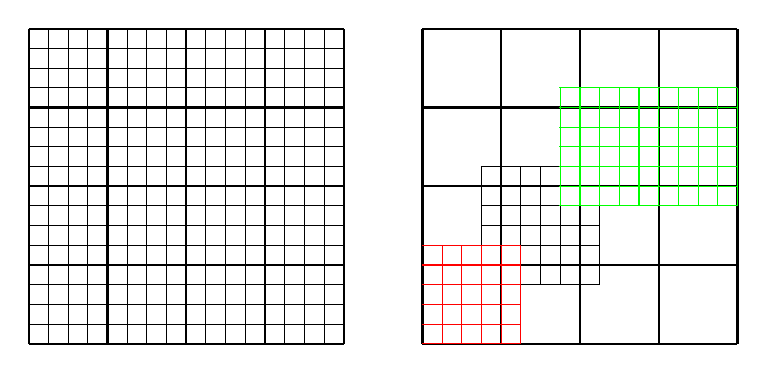
\begin{tikzpicture}
    \draw[step=.25cm] (-2,-2) grid (2,2);
    \draw[step=1cm,thick] (-2,-2) grid (2,2);
    \draw[step=1cm,thick] (3,-2) grid (7,2);
    \draw[step=.25cm] (3.74,-1.25) grid (5.25,0.25);
    \draw[step=.25cm,red] (3,-2) grid (4.25,-0.75);
    \draw[step=.25cm,green] (4.74,-0.25) grid (7,1.25);
  \end{tikzpicture}
  \caption{Fine mesh and coarse mesh (left) for overlapping domain
    decomposition. Examples for a subdomain decomposition on the
    right.}
  \label{fig:schwarz:ddmeshes}
\end{figure}

\begin{definition}
  A smooth \define{partition of unity} with respect to the subdomains
  $\Omega_1,\Omega_2,\dots,\Omega_J$ of $\Omega$ is a set of
  nonnegative functions $\{\phi_1,\dots,\phi_J\}\subset
  C^\infty(\overline\Omega)$ such that
  \begin{xalignat}2
    \label{eq:schwarz:6}
    \phi_j(x) &  = 0
    & \forall x & \in \Omega\setminus\Omega_j, \quad j=1,\dots,J
    \\
    \label{eq:schwarz:7}
    \sum_{j=1}^J \phi_j(x) &= 1
    & \forall x&\in\overline\Omega.
  \end{xalignat}
  Furthermore, we assume that there is a positive constant $\delta$,
  called \define{overlap}, such that for all $j=1,\dots,J$ there holds
  \begin{gather}
    \label{eq:schwarz:8}
    \norm{\nabla\phi j}_{L^\infty(\Omega)} \lesssim \frac 1\delta,
  \end{gather}
  where the implicit constant is independent of $h$, $\delta$ and $J$.
\end{definition}

\begin{note}
  The term overlap for $\delta$ is justified by the following
  consideration. Let $x \in \Omega_j$ be a point which is not in any
  other $\Omega_i$. Then, $\phi_j(x) = 1$. If~\eqref{eq:schwarz:8} is
  to hold, then it is necessary
  $\operatorname{dist}(x,\partial\Omega_J) \ge \delta$ (up to a
  constant, but this constant is already
  in~\eqref{eq:schwarz:8}). Thus, the points of distance less than
  $\delta$ from $\partial\Omega_j$ must be elements of another
  subdomain as well, which is then said to overlap with $\Omega_j$.
\end{note}

\begin{notation}
  The solution space of our problem is the space $V=V_h$ given by the
  finite element space on the mesh $\T_h$. Since the meshes are
  nested, the finite element space $V_0 \equiv V_H$ on the mesh $\T_H$ is a
  subspace of $V_h$. Additionally, we define finite element spaces on
  $\Omega_j$ by
  \begin{gather}
    \label{eq:schwarz:9}
    V_j = \bigl\{ v\in V_h \big| \forall x\in\Omega\setminus\Omega_j :
    v(x) =0\bigr\}.
  \end{gather}
\end{notation}

\begin{definition}
  Let the spaces $V_j$, $j=0,\dots,J$ be defined as above. Then, the
  \define{two-level Schwarz preconditioner} is defined as
  \begin{gather}
    \label{eq:schwarz:10}
    B_{\text{TLS}} = \sum_{j=0}^J P_j A^{-1} = \sum_{j=0}^J A_j^{-1} \Pi_j,
  \end{gather}
  where $P_j$ is defined according to~\eqref{eq:schwarz:2} and $A_j:
  V_j\to V_j^*$ by
  \begin{gather}
    \scal(A_j u_j, v_j)_V = a(u_j, v_j),\quad\forall u_j, v_j \in V_j.
  \end{gather}
\end{definition}

\begin{note}
  In order to simplify notation, we have assigned index zero to
  $V_H$. Thus, sums in future terms may either start at one, summing
  over subdomains, or at zero, summing over all subspaces.
\end{note}

\begin{lemma}
  There holds
  \begin{gather}
    \label{eq:schwarz:11}
    V_h = \sum_{j=1}^J V_j.
  \end{gather}
\end{lemma}

\begin{proof}
  Let $I_h: C(\overline\Omega) \to V_h$ be the interpolation operator
  of the finite element space. Then, for any given $v\in V_h$ define
  $v_j = I_h(\phi_j v)$, where $\phi_j$ is the function associated to
  $\Omega_j$ of a partition of unity for $\Omega_1,\dots,\Omega_J$.
  
  By definition of $\phi_j$, there holds $\phi_j v = 0$ on
  $\Omega\setminus\Omega_j$. Furthermore, we assumed that a mesh cell
  of $\T_h$ is either completely in $\Omega_j$ or completely in its
  complement. Since nodal values of a cell are located in the cell
  itself, this implies that $I_h (\phi_j v) = 0$ on
  $\Omega\setminus\Omega_j$. Therefore, $I_h (\phi_j v) \in V_j$.
  
  On the other hand, we use the linearity of the interpolation
  operator to obtain
  \begin{gather*}
    \sum_{j=1}^J v_j = \sum_{j=1}^J I_h(\phi_j v)
    = I_h\left(v\sum_{j=1}^J \phi_h\right)
    = I_h v = v,
  \end{gather*}
  thus, the $v_j$ are indeed a decomposition of $v$. Since $v\in V_h$
  was chosen arbitrarily, the lemma is proven.
\end{proof}

\begin{intro}
  The following lemmas serve to verify the assumptions of the abstract
  Theorem~\ref{???}.
\end{intro}

\begin{lemma}[Stable decomposition]
  \label{lemma:schwarz:stable-decomposition}
  Let $v_j\in V_j$ for $j=0,\dots,J$ be a composition of $v\in V_h$
  such that
  \begin{gather*}
    v=\sum_{j=0}^J v_j.
  \end{gather*}
  Then,
  \begin{gather}
    \label{eq:schwarz:12}
    a(v,v) \lesssim \sum_{j=0}^J a(v_j, v_j).
  \end{gather}
\end{lemma}

\begin{proof}
  \begin{todo}
    p. 187 f.
  \end{todo}
\end{proof}

\begin{lemma}
  For each $v\in V_h$ there exists a decomposition $v=\sum_{j=0}^J
  v_j$ with $v_j\in V_j$, such that
  \begin{gather}
    \label{eq:schwarz:13}
    \sum_{j=0}^J a(v_j, v_j)
    \lesssim \left(1+\frac H\delta\right)^2 a(v,v).
  \end{gather}
\end{lemma}

\begin{proof}
  \begin{todo}
    p. 189 f.
  \end{todo}
\end{proof}

\begin{theorem}
  \label{theorem:schwarz:two-level-convergence}
  Under the assumptions made so far in this section, there holds
  \begin{gather}
    \label{eq:schwarz:14}
    \kappa(B_{\text{TLS}} A_h)
    = \frac{\lambda(B_{\text{TLS}}, A_h)}{\Lambda(B_{\text{TLS}},
      A_h)}
    \lesssim \left(1+\frac H\delta\right)^2,
  \end{gather}
  where the implicit constant is independent of $h$, $\delta$, $H$, and $J$.
\end{theorem}

\begin{proof}
  \begin{todo}
    ...
  \end{todo}
\end{proof}

\begin{remark}
  \begin{todo}
    \begin{itemize}
    \item Size of overlap vs. numerical effort
    \item Size of overlap vs. coarse grid size
    \item Size of coarse grid and subdomains vs. speed
    \end{itemize}
  \end{todo}
\end{remark}

%%% Local Variables: 
%%% mode: latex
%%% TeX-master: "main"
%%% End: 


\chapter{Multigrid methods}

\begin{intro}
  \putindex{multigrid} Multigrid methods avoid the problems discussed
  in the section on two-level Schwarz methods by using not only two,
  but a whole hierarchy of mesh levels. On each level, an approximate
  solver, a so called smoother is employed, which improves the error
  somewhat, and then an approximation on a coarser level is used to
  improve further. This is done down to the coarsest level, where we
  assume that the solution process is cheap.
\end{intro}

\begin{definition}
  A \define{hierarchy of spaces} $\{V_\ell\}_0\le \ell \le L$ is a
  sequence of the form
  \begin{gather}
    V_0 \subset V_1 \subset \dots \subset V_L.
  \end{gather}
  We assume that $V_L = V$ is the high resolution space on which we
  want to solve~\eqref{eq:itintro:1}, but where the condition number
  of the matrix $\mat A$ is bad. On the other end of the spectrum, we
  assume that the solution of~\eqref{eq:itintro:1} on $V_0$ is easily
  possible.
\end{definition}

\begin{definition}
  A \define{multigrid method} consists of the following components:
  \begin{enumerate}
  \item A \define{smoother} $R_\ell$ acting on the level space
    $V_\ell$, usually an iterative method like Richardson, Jacobi,
    Gauss-Seidel or a Schwarz method.
  \item A \define{coarse grid solver} solving the problem on $V_0$
    exactly.
  \item Transfer operators between the levels $V_{\ell}$ and
    $V_{\ell+1}$. For standard finite element methods, this is
    typically the embedding operator. The transfer in opposite
    direction is achieved by the $L^2$-projection.
  \end{enumerate}
  
  On a given level $V_{\ell}$, the multigrid level consists of an
  alternating sequence of \putindex{smoothing step}s and
  \putindex{coarse grid correction}s, where the latter consist of a
  projection of the residual to the space $V_{\ell-1}$ and then
  recursive application of the same sequence. This is easiest
  described by the function
  \begin{subequations}
    \label{eq:mg:5}
  \begin{gather}
    \label{eq:mg:1}
    u_1 = MG_\ell(u^{(0)}, g),
  \end{gather}
  which takes an initial value $u^{(0)}$ and computes an approximation
  $u_1$ to the solution to $A_\ell u = g$ by the following scheme:
  first, for $\ell = 0$ let
  \begin{gather*}
    MG_0(u^{(0)}, g) = A_0^{-1} g_0.
  \end{gather*}
  On levels $\ell \neq 0$, perform the three steps
  \begin{itemize}
  \item Pre-smoothing: apply $m_{\text{pre}}$ steps of a Richardson
    iteration preconditioned with the smoother $R_\ell$:
    \begin{gather}
      \label{eq:mg:2}
      u^{(k+1)} = u^{(k)} - R_{\ell}^{-1} \left(A_\ell u^{(k)} - g_\ell\right),
      \qquad 0 \le k < m_{\text{pre}}.
    \end{gather}
    \item Coarse grid correction: let $v^{(0)} \in V_{\ell-1}$ and
      $g_{\ell-1} \in V_{\ell-1}^*$ such that
      \begin{gather}
        \label{eq:mg:3}
        g_{\ell-1} = \Pi_{\ell-1}^T \left(g_\ell - A_\ell u^{(m_{\text{pre}})}\right),
        \qquad
        v^{(0)} = 0.
      \end{gather}
      Then, compute 
      \begin{gather}
        \label{eq:mg:4}
        v^{(k+1)} = MG_{\ell-1}(v^{(k)}, g_{\ell-1}),
      \qquad 0 \le k < m_{\text{coarse}}.
      \end{gather}
      Let $w^{(0)} \in V_{\ell}$ be given by $w^{(0)} =
      u^{(m_{\text{pre}})} + v^{(m_{\text{coarse}})}$.
  \item Post-smoothing: apply $m_{\text{post}}$ steps of a Richardson
    iteration preconditioned with the smoother $R_\ell$:
    \begin{gather}
      \label{eq:mg:2a}
      w^{(k+1)} = w^{(k)} - R_{\ell}^{-1} \left(A_\ell w^{(k)} - g_\ell\right),
      \qquad 0 \le k < m_{\text{post}}.
    \end{gather}
    Assign $MG(u^{(0)}, g_\ell) = w^{(m_{\text{post}})}$.
  \end{itemize}    
  \end{subequations}
  
  This method has three parameters, the numbers of pre- and post
  smoothing steps $m_{\text{pre}}$ and $m_{\text{post}}$ as well as
  the number of coarse grid iterations $m_{\text{coarse}}$. Here, it
  is the last one which has a strong impact on the structure of the
  iteration. It defines what is called the \define{cycle type}, which
  is either \define{V-cycle} for $m_{\text{coarse}} = 1$ or
  \define{W-cycle} for $m_{\text{coarse}} = 2$. The structure of the
  cycles can be seen in Figure~\ref{fig:mg:1}.
\end{definition}
\begin{figure}[tp]
  \centering
  \begin{minipage}[t]{.49\linewidth}
  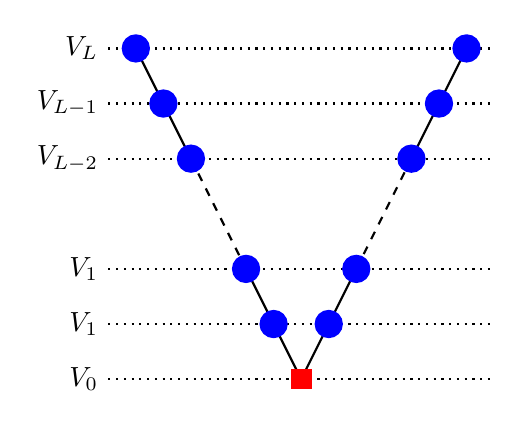
\begin{tikzpicture}[thick,scale=.7]
    % Levels
    \draw[dotted](0,0) node[anchor=east]{$V_0$} -- (7,0);
    \draw[dotted](0,1) node[anchor=east]{$V_1$} -- (7,1);
    \draw[dotted](0,2) node[anchor=east]{$V_1$} -- (7,2);
    \draw[dotted](0,4) node[anchor=east]{$V_{L-2}$} -- (7,4);
    \draw[dotted](0,5) node[anchor=east]{$V_{L-1}$} -- (7,5);
    \draw[dotted](0,6) node[anchor=east]{$V_L$} -- (7,6);
    
    % Transfers
    \draw(0.5,6) -- (1.5,4);
    \draw[dashed](1.5,4) -- (2.5,2);
    \draw(2.5,2) -- (3.5,0) -- (4.5,2);
    \draw[dashed](4.5,2) -- (5.5,4);
    \draw(5.5,4) -- (6.5,6);
    
    % Smoothers and coarse grid correction
    \node at (0.5,6) [circle,draw=blue,fill=blue] {};
    \node at (1.0,5) [circle,draw=blue,fill=blue] {};
    \node at (1.5,4) [circle,draw=blue,fill=blue] {};
    \node at (2.5,2) [circle,draw=blue,fill=blue] {};
    \node at (3.0,1) [circle,draw=blue,fill=blue] {};
    \node at (4.0,1) [circle,draw=blue,fill=blue] {};
    \node at (4.5,2) [circle,draw=blue,fill=blue] {};
    \node at (5.5,4) [circle,draw=blue,fill=blue] {};
    \node at (6.0,5) [circle,draw=blue,fill=blue] {};
    \node at (6.5,6) [circle,draw=blue,fill=blue] {};
    \node at (3.5,0) [rectangle,draw=red,fill=red] {};
  \end{tikzpicture}    
  \end{minipage}
  \begin{minipage}[t]{.49\linewidth}
  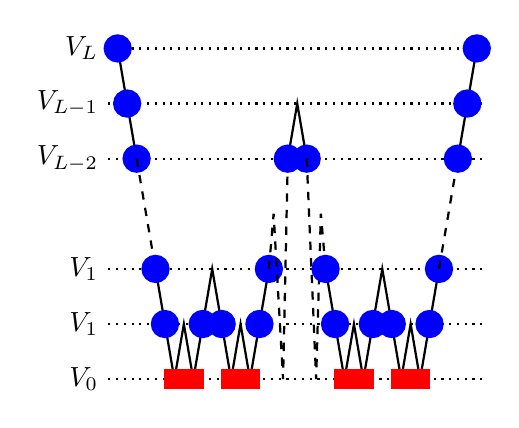
\begin{tikzpicture}[thick,yscale=.7,xscale=.6]
    % Levels
    \draw[dotted](0,0) node[anchor=east]{$V_0$} -- (8.0,0);
    \draw[dotted](0,1) node[anchor=east]{$V_1$} -- (8.0,1);
    \draw[dotted](0,2) node[anchor=east]{$V_1$} -- (8.0,2);
    \draw[dotted](0,4) node[anchor=east]{$V_{L-2}$} -- (8.0,4);
    \draw[dotted](0,5) node[anchor=east]{$V_{L-1}$} -- (8.0,5);
    \draw[dotted](0,6) node[anchor=east]{$V_L$} -- (8.0,6);

    % Transfers and smoothers
    \draw(0.2,6) node[circle,draw=blue,fill=blue] {}
    -- (0.4,5) node[circle,draw=blue,fill=blue] {}
    -- (0.6,4) node[circle,draw=blue,fill=blue] {};
    \draw[dashed](0.6,4) -- (1.0,2);
    \draw (1.0,2) node[circle,draw=blue,fill=blue] {}
    -- (1.2,1) node[circle,draw=blue,fill=blue] {}
    -- (1.4,0) node[rectangle,draw=red,fill=red] {}
    -- (1.6,1)
    -- (1.8,0) node[rectangle,draw=red,fill=red] {}
    -- (2.0,1) node[circle,draw=blue,fill=blue] {}
    -- (2.2,2)
    -- (2.4,1) node[circle,draw=blue,fill=blue] {}
    -- (2.6,0) node[rectangle,draw=red,fill=red] {}
    -- (2.8,1)
    -- (3.0,0) node[rectangle,draw=red,fill=red] {}
    -- (3.2,1) node[circle,draw=blue,fill=blue] {}
    -- (3.4,2) node[circle,draw=blue,fill=blue] {};
    \draw[dashed](3.4,2) -- (3.5,3) -- (3.7,0) -- (3.8,4);
    \draw(3.8,4) node[circle,draw=blue,fill=blue] {}
    -- (4.0,5)
    -- (4.2,4) node[circle,draw=blue,fill=blue] {};
    \draw[dashed] (4.2,4) -- (4.4,0) -- (4.5,3) 
    -- (4.6,2)
    ;
    \draw (4.6,2) node[circle,draw=blue,fill=blue] {}
    -- (4.8,1) node[circle,draw=blue,fill=blue] {}
    -- (5.0,0) node[rectangle,draw=red,fill=red] {}
    -- (5.2,1)
    -- (5.4,0) node[rectangle,draw=red,fill=red] {}
    -- (5.6,1) node[circle,draw=blue,fill=blue] {}
    -- (5.8,2)
    -- (6.0,1) node[circle,draw=blue,fill=blue] {}
    -- (6.2,0) node[rectangle,draw=red,fill=red] {}
    -- (6.4,1)
    -- (6.6,0) node[rectangle,draw=red,fill=red] {}
    -- (6.8,1) node[circle,draw=blue,fill=blue] {}
    -- (7.0,2) node[circle,draw=blue,fill=blue] {};
    \draw[dashed] (7.0,2) -- (7.4,4);
    \draw (7.4,4) node[circle,draw=blue,fill=blue] {}
    -- (7.6,5) node[circle,draw=blue,fill=blue] {}
    -- (7.8,6) node[circle,draw=blue,fill=blue] {};    
  \end{tikzpicture}    
  \end{minipage}
  \caption{Smoothing and grid transfer of the V-cycle (left) and
    W-cycle (right). Black lines indicate grid transfer, blue dots are
  smoothing operations and red squares are coarse grid
  solvers. ``Time'' is left to right.}
  \label{fig:mg:1}
\end{figure}

\begin{remark}
  Figure~\ref{fig:mg:1} shows that the recursive structure of the
  W-cycle is much more complex than that of the V-cycle. The
  complexity analysis below will show that higher values of
  $m_{\text{coarse}}$ do not lead to efficient algorithms.
\end{remark}

\begin{definition}
  If the numbers of pre- and post smoothing steps in the V-cycle are
  dependent on the level $\ell$, we speak of the \define{variable
    V-cycle}. A typical choice is $m_\ell = 2^{L-\ell} m_L$, thus
  doubling the number of smoothing steps whenever stepping down one
  level.
\end{definition}

\begin{note}
  The variable V-cycle with $m_\ell$ as mentioned in the previous
  definition has as many smoothing steps per iteration as the W-cycle.
\end{note}

\begin{remark}
  If we use an additive or multiplicative Schwarz method (omitting the
  coarse grid) as our smoother $R_\ell$, it should be possible in
  principle to use the analytical tools of
  Chapter~\ref{cha:iteration:schwarz-methods}. The difficulty then
  consists in ensuring that the spectral radius of the iteration
  matrix does not grow towards one if we proceed upwards on our scale
  of spaces $V_\ell$. This remark is a todo for the author and an
  encouragement for the reader. Hints may be found
  in~\cite{GriebelOswald95,Xu92}.
\end{remark}

\begin{remark}
  It turns out that the techniques used for the analysis of the
  V-cycle and the W-cycle, respectively are quite
  different. Therefore, we separate them into two sections.
\end{remark}

\begin{theorem}
  Let $n_\ell$ be the dimension of $V_\ell$. Assume that the effort
  needed to for the operations in equations~\eqref{eq:mg:5}b/c/e is
  linear in $n_\ell$ and assume that $ n_{\ell+1}/n_\ell \approx 2^d$,
  where $d$ is the space dimension of the grid. Assume that the effort
  for the coarse grid solver is negligible. Then, the effort for
  one step of the V-cycle is of order $n_L$. The effort for one step
  of the W-cycle is of order $n_L$ for $d \ge 2$, while it is of order
  $n_L \log(n_L)$ in one dimension.
\end{theorem}

\begin{proof}
  Start the recursion on level $L$ with the function $MG_L(0,
  g)$. This function calls $MG_{L-1}(\ldots)$ $m_{\text{coarse}}$
  times. Thus, by recursion, $MG_{\ell}(\ldots)$ is executed
  $m_{\text{coarse}}^{L-\ell}$ times.
  
  By our assumptions, the amount of operations $\breve N_\ell$ in $MG_\ell(\ldots)$
  without the coarse grid correction is linear in $n_\ell$, say
  bounded by $Cn_\ell$. Then, the overall effort $N_L$ on level $L$ is
  \begin{gather}
    \label{eq:mg:6}
    N_L \le C \sum_{\ell=1}^L n_\ell m_{\text{coarse}}^{L-\ell} \le C
    \sum_{\ell=1}^L n_L 2^{d(l-L)}m_{\text{coarse}}^{L-\ell}
    = C n_L \sum_{\ell=1}^L \left(\frac{m_{\text{coarse}}}{2^d}\right)^l.
  \end{gather}
  It remains to notice that the sum converges and is bounded
  independent of $L$ if and only if $m_{\text{coarse}}/2^d < 1$. The
  statements of the theorem follow immediately, observing that $L
  \simeq \log n_L$.
\end{proof}

\begin{lemma}
  Let $B_\ell^{-1}$ be the operator associated with the action of the
  multigrid preconditioner on level $\ell$ for
  $\ell=0,\ldots,L$. Then, the error after one step of the multigrid
  method has the form
  \begin{gather}
    \label{eq:mg:7}
    u^{(k+1)} - u = E_L \left(u^{(k)} - u \right),
  \end{gather}
  where for $\ell=0,\ldots,L$ we denote by $E_\ell$ the
  \putindex{error propagation operator}
  \begin{gather}
    \label{eq:mg:8}
    E_\ell = \left(I-R_\ell^{-1} A_\ell\right)^{m_{\text{post}}}
    \left(I-B_{\ell-1}^{-1}A_{\ell-1} P_{\ell-1}\right)^{m_{\text{coarse}}}
     \left(I-R_\ell^{-1} A_\ell\right)^{m_{\text{pre}}}
  \end{gather}
\end{lemma}

\begin{proof}
  For the smoother, we use the standard technique for Richardson's
  method outlined in Lemma~\ref{lemma:richardson:1}. For the coarse
  grid correction, we use Lemma~\ref{lemma:schwarz:2}.
\end{proof}

\begin{note}
  The structure of the error propagation operator~\eqref{eq:mg:8}
  already suggests the course of the multigrid analysis (as well as
  the design of smoothers). Namely, we will have to decompose $V_l$
  into $V_{l-1}$ and its $A$-orthogonal complement. Then, we use the
  induction argument that $I-B_{\ell-1}^{-1}A_{\ell-1}$ is is small on
  $V_{l-1}$, while bounded on its complement. Vice versa,
  $I-R_\ell^{-1} A_\ell$ must be bounded on all of $V_\ell$, while
  providing good reduction properties on the complement of $V_{l-1}$.
\end{note}

\section{The V-cycle}

\begin{assumption}
  \label{assumption:mg:1}
  Let the smoother $R_\ell$ be symmetric, positive definite and let
  the following two conditions hold, the second for some positive
  constant $\alpha$ independent of $\ell$:
  \begin{subequations}
    \label{eq:mg:9}
    \begin{xalignat}{2}
      \label{eq:mg:10}
      a\bigl((I-R_\ell^{-1}A_\ell)v,v\bigr) & \ge 0
      & \forall v &\in V_\ell, \\
      \label{eq:mg:20}
      r(w,w) &\le \alpha a(w,w)
      & \forall v &\in V_\ell, \quad w = (I-P_{\ell-1}) v
    \end{xalignat}
  \end{subequations}
\end{assumption}

\begin{theorem}
  Let $a(.,.)$ be symmetric, positive definite and let
  Assumption~\ref{assumption:mg:1} hold. Then, the V-cycle operator
  with $m_{\text{pre}} =m_{\text{post}} = m$ admits the estimate
  \begin{gather}
    \label{eq:mg:11}
    0 \le a(\bigl((I-B_\ell^{-1}A_\ell)v,v\bigr) \le \delta a(v,v),
    \qquad \forall v \in V_\ell,
  \end{gather}
  where
  \begin{gather}
    \label{eq:mg:12}
    \delta = \frac{\alpha}{\alpha+2m}.
  \end{gather}
  In particular, the contraction number of the multigrid method is
  bounded by a number less than 1, independent of the level.
\end{theorem}

\begin{proof}
  \footnote{This version of the proof is taken
    from~\cite{ArnoldFalkWinther97Hdiv}. It can also be found
    in~\cite{BraessHackbusch83,Bramble93}.}
  First, abbreviate $K_{\ell} = I-R_{\ell}^{-1} A_\ell$, the error
  propagation operator of a smoothing step. Now we will prove the
  theorem by induction over $\ell$. First, since $B_0 = A_0$, it holds
  on level zero. For higher levels, we derive from~\eqref{eq:mg:8} the
  relation
  \begin{gather}
    \label{eq:mg:13}
    E_\ell = I-B_\ell^{-1} A_\ell = K_\ell^m\Bigl(
    (I-P_{\ell-1}) + (I-B_{\ell-1}^{-1} A_{\ell-1}) P_{\ell-1}
    \Bigr) K_\ell^m.
  \end{gather}
  Non-negativity follows readily by the induction argument and
  the same properties of the smoother and the Ritz-projection. For the
  upper bound, let $w = K_\ell^m v$ to obtain by the induction
  hypothesis
  \begin{multline}
    \label{eq:mg:14}
    a(E_\ell v,v) \le a\bigl((I-P_{\ell-1}) w,w\bigr) + \delta
    a(P_{\ell-1}w,w)
    \\
    = (1-\delta) a\bigl((I-P_{\ell-1}) w,w\bigr)
   + \delta a(w,w).
  \end{multline}
  Now we use the smoothing hypothesis anf the
  Bunyakovsky-Cauchy-Schwarz inequality for the bilinear form $r(.,.)$
  associated with the smoothing operator $R_\ell$ to obtain
  \begin{align*}
    a\bigl((I-P_{\ell-1}) w,w\bigr)
    &= \scal({(I-P_{\ell-1}) w}, A_\ell w) \\
    &= \scal(R_\ell {(I-P_{\ell-1})} w, R_\ell^{-1} A_\ell w)
    \\
    &= r\bigl((I-P_{\ell-1}) w, R_\ell^{-1} A_\ell w\bigr) \\
    &\le \sqrt{r\bigl((I-P_{\ell-1}) w,(I-P_{\ell-1}) w\bigr)}
    \sqrt{r\bigl(R_\ell^{-1} A_\ell w, R_\ell^{-1} A_\ell w\bigr)}
    \\
    &\le \sqrt{\alpha a\bigl((I-P_{\ell-1}) w,(I-P_{\ell-1}) w\bigr)}
    \sqrt{a\bigl(R_\ell^{-1} A_\ell w, w\bigr)}
  \end{align*}
  Using the projection property of $I-P_{\ell-1}$, we obtain
  \begin{gather}
    \label{eq:mg:15}
    a\bigl((I-P_{\ell-1}) w,w\bigr) \le \alpha a\bigl(R_\ell^{-1} A_\ell
    w, w\bigr)
    = \alpha a\bigl((I-K_\ell) K_\ell^{2m} v,v\bigr).
  \end{gather}
  
  The smoothing assumption also guarantees that the spectrum of
  $K_\ell$ is contained in the interval $[0,1]$. Therefore,
  \begin{gather}
    \label{eq:mg:16}
    a\bigl((I-K_\ell) K_\ell^{2m} v,v\bigr)
    \le a\bigl((I-K_\ell) K_\ell^{i} v,v\bigr),
    \qquad i=0,\dots,2m,
  \end{gather}
  yielding by deflating the telescoping sum
  \begin{gather}
    \label{eq:mg:17}
    a\bigl((I-K_\ell) K_\ell^{2m} v,v\bigr)
    \le \frac1{2m} \sum_{i=0}^{2m-1}
    a\bigl((I-K_\ell) K_\ell^{i} v,v\bigr)
    = \frac1{2m} a\bigl((I-K_\ell^{2m}) v,v\bigr)
  \end{gather}
  Combining~\eqref{eq:mg:14}, \eqref{eq:mg:15}, and~\eqref{eq:mg:17},
  we obtain
  \begin{gather}
    \begin{split}
      a(E_\ell v,v) &\le (1-\delta)\frac\alpha{2m}
      a\bigl((I-K_\ell^{2m}) v,v\bigr)
      + \delta a(K_\ell^m v,K_\ell^m v)
      \\
      &= (1-\delta)\frac\alpha{2m} a(v,v)
      + \left(\delta - (1-\delta)\frac\alpha{2m}\right)
      a(K_\ell^m v,K_\ell^m v).
    \end{split}
  \end{gather}
  Finally, we enter $\delta=\alpha/(\alpha+2m)$ to obtain
  \begin{gather*}
    \delta - (1-\delta)\frac\alpha{2m} = 0,
  \end{gather*}
  and thus
  \begin{gather}
    \label{eq:mg:18}
    a(E_\ell v,v) \le \left(1-\frac\alpha{\alpha+2m}\right)\frac\alpha{2m}
    a(v,v) = \frac\alpha{\alpha+2m}a(v,v). 
  \end{gather}
\end{proof}

\begin{lemma}
  Let $R_\ell$ be the scaled additive Schwarz method
  \begin{gather}
    \label{eq:mg:19}
    R_a^{-1} = \omega \sum_{j=1}^J P_j A^{-1},
  \end{gather}
  where the subspaces $V_j$ are defined by overlapping subdomains
  $\Omega_j$ as in~\eqref{eq:schwarz:9}. Not that we do not include
  the coarse space here. Then, for $\omega$ sufficiently small, this
  smoother fulfills Assumption~\ref{assumption:mg:1}.
\end{lemma}

\begin{proof}
  The positive definiteness and symmetry of the smoother have been
  proven in an abstract way in Lemma~\ref{lemma:schwarz:3}. In order
  to prove estimate~\eqref{eq:mg:10}, we observe that by
  Lemma~\ref{lemma:schwarz:5} and Lemma~\ref{lemma:schwarz:6}
  \begin{gather*}
    r(v,v) = \omega \min_{v=\sum v_j} a(v_j, v_j) \gtrsim \omega a(v,v),
  \end{gather*}
  where the implicit constant depends on the number of overlaps in
  Definition~\ref{definition:schwarz:finite-covering}. Thus, we can
  choose $\omega$ independent of $\ell$ such that
  \begin{gather*}
    r(v,v) \ge a(v,v) \qquad \forall v\in V_\ell.
  \end{gather*}
  Accordingly, $R_\ell - A_\ell$ is positive definite, and since
  $R_\ell^{-1}$ is as well, so is $I-R_\ell^{-1} A_\ell$.
  It remains to prove~\eqref{eq:mg:20}, but this is exactly the second
  half of the proof of Lemma~\ref{lemma:schwarz:stable-decomposition},
  if we replace the Clément interpolant into the coarse space by the
  Ritz projection.
\end{proof}

%\section{The W-cycle and two-grid convergence}


%%% Local Variables: 
%%% mode: latex
%%% TeX-master: "main"
%%% End: 


\printbibliography
\printindex
\end{document}


%%% Local Variables: 
%%% mode: latex
%%% TeX-master: "main"
%%% End: 
